\documentclass[twoside]{book}

% Packages required by doxygen
\usepackage{fixltx2e}
\usepackage{calc}
\usepackage{doxygen}
\usepackage[export]{adjustbox} % also loads graphicx
\usepackage{graphicx}
\usepackage[utf8]{inputenc}
\usepackage{makeidx}
\usepackage{multicol}
\usepackage{multirow}
\PassOptionsToPackage{warn}{textcomp}
\usepackage{textcomp}
\usepackage[nointegrals]{wasysym}
\usepackage[table]{xcolor}

% Font selection
\usepackage[T1]{fontenc}
\usepackage[scaled=.90]{helvet}
\usepackage{courier}
\usepackage{amssymb}
\usepackage{sectsty}
\renewcommand{\familydefault}{\sfdefault}
\allsectionsfont{%
  \fontseries{bc}\selectfont%
  \color{darkgray}%
}
\renewcommand{\DoxyLabelFont}{%
  \fontseries{bc}\selectfont%
  \color{darkgray}%
}
\newcommand{\+}{\discretionary{\mbox{\scriptsize$\hookleftarrow$}}{}{}}

% Page & text layout
\usepackage{geometry}
\geometry{%
  a4paper,%
  top=2.5cm,%
  bottom=2.5cm,%
  left=2.5cm,%
  right=2.5cm%
}
\tolerance=750
\hfuzz=15pt
\hbadness=750
\setlength{\emergencystretch}{15pt}
\setlength{\parindent}{0cm}
\setlength{\parskip}{3ex plus 2ex minus 2ex}
\makeatletter
\renewcommand{\paragraph}{%
  \@startsection{paragraph}{4}{0ex}{-1.0ex}{1.0ex}{%
    \normalfont\normalsize\bfseries\SS@parafont%
  }%
}
\renewcommand{\subparagraph}{%
  \@startsection{subparagraph}{5}{0ex}{-1.0ex}{1.0ex}{%
    \normalfont\normalsize\bfseries\SS@subparafont%
  }%
}
\makeatother

% Headers & footers
\usepackage{fancyhdr}
\pagestyle{fancyplain}
\fancyhead[LE]{\fancyplain{}{\bfseries\thepage}}
\fancyhead[CE]{\fancyplain{}{}}
\fancyhead[RE]{\fancyplain{}{\bfseries\leftmark}}
\fancyhead[LO]{\fancyplain{}{\bfseries\rightmark}}
\fancyhead[CO]{\fancyplain{}{}}
\fancyhead[RO]{\fancyplain{}{\bfseries\thepage}}
\fancyfoot[LE]{\fancyplain{}{}}
\fancyfoot[CE]{\fancyplain{}{}}
\fancyfoot[RE]{\fancyplain{}{\bfseries\scriptsize Generated by Doxygen }}
\fancyfoot[LO]{\fancyplain{}{\bfseries\scriptsize Generated by Doxygen }}
\fancyfoot[CO]{\fancyplain{}{}}
\fancyfoot[RO]{\fancyplain{}{}}
\renewcommand{\footrulewidth}{0.4pt}
\renewcommand{\chaptermark}[1]{%
  \markboth{#1}{}%
}
\renewcommand{\sectionmark}[1]{%
  \markright{\thesection\ #1}%
}

% Indices & bibliography
\usepackage{natbib}
\usepackage[titles]{tocloft}
\setcounter{tocdepth}{3}
\setcounter{secnumdepth}{5}
\makeindex

% Hyperlinks (required, but should be loaded last)
\usepackage{ifpdf}
\ifpdf
  \usepackage[pdftex,pagebackref=true]{hyperref}
\else
  \usepackage[ps2pdf,pagebackref=true]{hyperref}
\fi
\hypersetup{%
  colorlinks=true,%
  linkcolor=blue,%
  citecolor=blue,%
  unicode%
}

% Custom commands
\newcommand{\clearemptydoublepage}{%
  \newpage{\pagestyle{empty}\cleardoublepage}%
}

\usepackage{caption}
\captionsetup{labelsep=space,justification=centering,font={bf},singlelinecheck=off,skip=4pt,position=top}

%===== C O N T E N T S =====

\begin{document}

% Titlepage & ToC
\hypersetup{pageanchor=false,
             bookmarksnumbered=true,
             pdfencoding=unicode
            }
\pagenumbering{roman}
\begin{titlepage}
\vspace*{7cm}
\begin{center}%
{\Large My Project }\\
\vspace*{1cm}
{\large Generated by Doxygen 1.8.11}\\
\end{center}
\end{titlepage}
\clearemptydoublepage
\tableofcontents
\clearemptydoublepage
\pagenumbering{arabic}
\hypersetup{pageanchor=true}

%--- Begin generated contents ---
\chapter{File Index}
\section{File List}
Here is a list of all documented files with brief descriptions\+:\begin{DoxyCompactList}
\item\contentsline{section}{\hyperlink{TaskB_8cc}{Task\+B.\+cc} \\*This is a program that count the how many lines and characters that is in the file }{\pageref{TaskB_8cc}}{}
\end{DoxyCompactList}

\chapter{File Documentation}
\hypertarget{TaskB_8cc}{}\section{Task\+B.\+cc File Reference}
\label{TaskB_8cc}\index{Task\+B.\+cc@{Task\+B.\+cc}}


This is a program that count the how many lines and characters that is in the file.  


{\ttfamily \#include $<$iostream$>$}\\*
{\ttfamily \#include $<$string$>$}\\*
{\ttfamily \#include $<$fstream$>$}\\*
Include dependency graph for Task\+B.\+cc\+:
\nopagebreak
\begin{figure}[H]
\begin{center}
\leavevmode
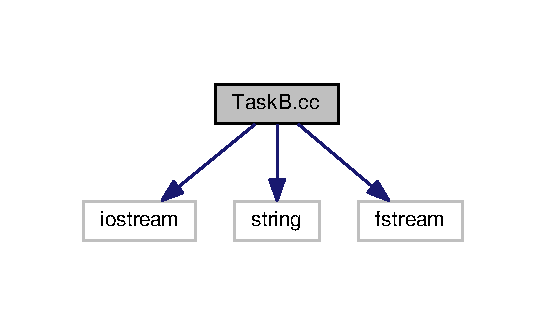
\includegraphics[width=262pt]{TaskB_8cc__incl}
\end{center}
\end{figure}
\subsection*{Functions}
\begin{DoxyCompactItemize}
\item 
int \hyperlink{TaskB_8cc_ad29c593e0c4993192080b49fee81b71c}{count\+Line} (char $\ast$p\+Name)
\begin{DoxyCompactList}\small\item\em count number of lines \end{DoxyCompactList}\item 
int \hyperlink{TaskB_8cc_a0f2a712f59874c79969f1ea5d8fcaab3}{count\+Char} (char $\ast$p\+Name)
\begin{DoxyCompactList}\small\item\em count number of characters \end{DoxyCompactList}\item 
int \hyperlink{TaskB_8cc_a0ddf1224851353fc92bfbff6f499fa97}{main} (int argc, char $\ast$argv\mbox{[}$\,$\mbox{]})
\begin{DoxyCompactList}\small\item\em count the number of lines and characters \end{DoxyCompactList}\end{DoxyCompactItemize}


\subsection{Detailed Description}
This is a program that count the how many lines and characters that is in the file. 

\begin{DoxyAuthor}{Author}
Bohong Li 
\end{DoxyAuthor}
\begin{DoxyDate}{Date}
2017/12/12 
\end{DoxyDate}


\subsection{Function Documentation}
\index{Task\+B.\+cc@{Task\+B.\+cc}!count\+Char@{count\+Char}}
\index{count\+Char@{count\+Char}!Task\+B.\+cc@{Task\+B.\+cc}}
\subsubsection[{\texorpdfstring{count\+Char(char $\ast$p\+Name)}{countChar(char *pName)}}]{\setlength{\rightskip}{0pt plus 5cm}int count\+Char (
\begin{DoxyParamCaption}
\item[{char $\ast$}]{p\+Name}
\end{DoxyParamCaption}
)}\hypertarget{TaskB_8cc_a0f2a712f59874c79969f1ea5d8fcaab3}{}\label{TaskB_8cc_a0f2a712f59874c79969f1ea5d8fcaab3}


count number of characters 


\begin{DoxyParams}{Parameters}
{\em p\+Name} & \\
\hline
\end{DoxyParams}
\begin{DoxyReturn}{Returns}
number of characters 
\end{DoxyReturn}
\index{Task\+B.\+cc@{Task\+B.\+cc}!count\+Line@{count\+Line}}
\index{count\+Line@{count\+Line}!Task\+B.\+cc@{Task\+B.\+cc}}
\subsubsection[{\texorpdfstring{count\+Line(char $\ast$p\+Name)}{countLine(char *pName)}}]{\setlength{\rightskip}{0pt plus 5cm}int count\+Line (
\begin{DoxyParamCaption}
\item[{char $\ast$}]{p\+Name}
\end{DoxyParamCaption}
)}\hypertarget{TaskB_8cc_ad29c593e0c4993192080b49fee81b71c}{}\label{TaskB_8cc_ad29c593e0c4993192080b49fee81b71c}


count number of lines 


\begin{DoxyParams}{Parameters}
{\em p\+Name} & \\
\hline
\end{DoxyParams}
\begin{DoxyReturn}{Returns}
number of lines 
\end{DoxyReturn}
\index{Task\+B.\+cc@{Task\+B.\+cc}!main@{main}}
\index{main@{main}!Task\+B.\+cc@{Task\+B.\+cc}}
\subsubsection[{\texorpdfstring{main(int argc, char $\ast$argv[])}{main(int argc, char *argv[])}}]{\setlength{\rightskip}{0pt plus 5cm}int main (
\begin{DoxyParamCaption}
\item[{int}]{argc, }
\item[{char $\ast$}]{argv\mbox{[}$\,$\mbox{]}}
\end{DoxyParamCaption}
)}\hypertarget{TaskB_8cc_a0ddf1224851353fc92bfbff6f499fa97}{}\label{TaskB_8cc_a0ddf1224851353fc92bfbff6f499fa97}


count the number of lines and characters 

\begin{DoxySeeAlso}{See also}
\hyperlink{TaskB_8cc_ad29c593e0c4993192080b49fee81b71c}{count\+Line()} 

\hyperlink{TaskB_8cc_a0f2a712f59874c79969f1ea5d8fcaab3}{count\+Char()} 
\end{DoxySeeAlso}

%--- End generated contents ---

% Index
\backmatter
\newpage
\phantomsection
\clearemptydoublepage
\addcontentsline{toc}{chapter}{Index}
\printindex

\end{document}
